\documentclass[11pt,a4paper]{article}

\usepackage[a4paper,left=2.0cm,right=2.0cm,top=1.55cm,bottom=1.55cm]{geometry}
\usepackage[T1]{fontenc}
\usepackage{lmodern}
\usepackage{graphicx}
\usepackage{xcolor}
\usepackage{array}
\usepackage{tabularx}
\usepackage{ragged2e}
\usepackage{enumitem}
\usepackage{fancyhdr}
\usepackage{tikz}
\usepackage{float}
\usetikzlibrary{shapes.geometric,arrows.meta,positioning,calc}
\usepackage{setspace}

% -------------------------------------------------
% COLOURS
% -------------------------------------------------
\definecolor{TitleBlue}{RGB}{61,103,154}

% -------------------------------------------------
% GENERAL SETTINGS
% -------------------------------------------------
\setlength{\parindent}{0pt}
\setlength{\parskip}{0pt}
\renewcommand{\arraystretch}{1.0}

\newcommand{\blueheading}[1]{%
    {\sffamily\color{TitleBlue}\fontsize{15}{18}\selectfont #1}%
}

\newcommand{\bluebigheading}[1]{%
    {\sffamily\bfseries\color{TitleBlue}\fontsize{16}{19}\selectfont #1}%
}

\newcommand{\instruction}[1]{%
    {\itshape\fontsize{10.5}{12.5}\selectfont #1}%
}

% Dynamic answerbox definition
\newcommand{\answerbox}[2][3.0cm]{%
    \vspace{2pt}
    \noindent
    \fbox{%
        \begin{minipage}[t]{\dimexpr\textwidth-2\fboxsep-2\fboxrule\relax}
            \vspace{2mm}
            \normalfont\fontsize{10.5}{13}\selectfont #2
            \vspace{2mm}
        \end{minipage}
    }
}

% -------------------------------------------------
% HEADER / FOOTER
% -------------------------------------------------
\pagestyle{fancy}
\fancyhf{}
\renewcommand{\headrulewidth}{0pt}
\renewcommand{\footrulewidth}{0pt}

\fancyhead[L]{%
    \sffamily\bfseries\itshape\fontsize{10.5}{12}\selectfont
    BTECH CSE DSCPP-III-2026-T278
}
\fancyhead[R]{%
    \sffamily\bfseries\fontsize{10.5}{12}\selectfont
    PROJECT PROPOSAL
}
\fancyfoot[R]{%
    \itshape\fontsize{10}{12}\selectfont
    Page \thepage
}
\setlength{\headheight}{14pt}
\setlength{\headsep}{23pt}
\setlength{\footskip}{24pt}

% -------------------------------------------------
% DOCUMENT
% -------------------------------------------------
\begin{document}

\vspace*{4mm}

\bluebigheading{PROJECT AND TEAM INFORMATION}

\vspace{8mm}

\begin{minipage}{\textwidth}
\blueheading{Project Title}

\vspace{1mm}

\answerbox[1.0cm]{RouteLens: Multiple Routes Visualization and Optimization system}
\end{minipage}

\vspace{8mm}

\blueheading{Student / Team Information}

\vspace{2mm}

% Team information table
\noindent
\begin{tabularx}{\textwidth}{|>{\RaggedRight\arraybackslash}p{0.69\textwidth}|>{\RaggedRight\arraybackslash}X|}
\hline
\begin{minipage}[t]{\linewidth}
\vspace{1.5mm}
\textit{Team Name:}\\[-1mm]
\textit{Team \#}
\vspace{1.5mm}
\end{minipage}
&
\begin{minipage}[t]{\linewidth}
\vspace{1.5mm}
\textit{Carpe Diem}
\\
\textit{DSCPP-III-2026-T278}
\end{minipage}
\\
\hline
\begin{minipage}[t][3.25cm][t]{\linewidth}
\vspace{1.5mm}
\textbf{Team member 1 (Team Lead)}\\[-1mm]
\textit{}
\vspace{2.0cm}
\end{minipage}
&
\begin{minipage}[t][3.25cm][t]{\linewidth}
\vspace{1.5mm}
\textit{Upreti Gunjita   2510382973}\\
\textit{2510382973@geu.ac.in}

\vspace{2mm}
\includegraphics[width=3.0cm,height=1.5cm,keepaspectratio]{gunjita.jpeg.png}
\end{minipage}
\\
\hline
\begin{minipage}[t][3.25cm][t]{\linewidth}
\vspace{1.5mm}
\textbf{Team member 2}\\[-1mm]
\textit{}
\vspace{2.0cm}
\end{minipage}
&
\begin{minipage}[t][3.25cm][t]{\linewidth}
\vspace{1.5mm}
\textit{Rawat Sneha , 2510012141}\\
\textit{2510012141@geu.ac.in}

\vspace{2mm}
\includegraphics[width=3.0cm,height=1.5cm,keepaspectratio]{sneha.jpeg.png}
\end{minipage}
\\
\hline
\begin{minipage}[t][3.25cm][t]{\linewidth}
\vspace{1.5mm}
\textbf{Team member 3}\\[-1mm]
\textit{}
\vspace{2.0cm}
\end{minipage}
&
\begin{minipage}[t][3.25cm][t]{\linewidth}
\vspace{1.5mm}
\textit{Rawat Aayush   2510370528}\\
\textit{2510370528@geu.ac.in}

\vspace{2mm}
\includegraphics[width=3.0cm,height=1.5cm,keepaspectratio]{aayush.jpeg.png}
\end{minipage}
\\
\hline
\end{tabularx}

\newpage

% -------------------------------------------------
% PAGE 2
% -------------------------------------------------

\bluebigheading{PROPOSAL DESCRIPTION (10 pts)}

\vspace{8mm}

\noindent\begin{minipage}{\textwidth}
\blueheading{Motivation (1 pt)}

\vspace{1mm}

\answerbox[8 cm]{Traffic jam is a problem in cities that is rapidly growing fast in the cities and especially during busy times when there are a lot of cars on the road. It is only growing with no escape out. This can be due to a lot of factrs and whether it be por condition of the roads or due to accidents or blocked roads or sudden changes in traffic. One can certainly not control the trafic but surely find a path that have lesser traffic relatively and  like the said "escape route" and to solve this we have brought "RouteLens".
"RouteLenss" is designed to help peopl to find the right path to travel and  that is low on trafic and saves one's time.
Because it let users to check each route individualy and they can examine several diferent possible routes to the destined stop on the map simultenously.
All routes will be represented in different colors.
This would allow the routes to be evaluated in a more useful manner as each shown route will have an info box showing details such as the length of the journey and, distance and amount of traffic jam and number of traffic lights.
The best route can be chosen by the user accordingly.
People will still be able to see the other options as wel and next to one another for easy comparison.
That give users the chance to investigate the various uses of each route and its possible limitations prior to comitting to one.
The system will treat the roads as a graph where the junction of the roads are the vertice and the roads are the lines betwen them.
Factors like driving time and traffic volume will be used to establish the weights of the lines.
The project will showcase the use of data structures and algorithms like graphs and queus and priority queues and linked lists and and shortest-path techniques.
RouteLens will make it easier for the driver to channel through the traffic easily by packing out a relatively leser traffic path.}
\end{minipage}

\vspace{8mm}

\noindent\begin{minipage}{\textwidth}
\blueheading{State of the Art / Current solution (1 pt)}

\vspace{1mm}

\answerbox[6cm]{Modern day navigation aplications such as Google Maps and Waze give route recomendations by using maps GPS data and traffic information and estimated travel times. They provide information about the routes with details like distance and travel time and traffic conditions.
However, in order to see the information user generally have to click at each route seprately and which makes it inconvenient to compare all the route simultaneously for beter decision-making. RouteLens solves this problem by using a visually interactive approach.
The user enters a start point and the destination and the RouteLens finds the best routes and shows them all on one map and displayed in diferent color.
Each route includes an information box that displays the estimated travel time (ETA) and  distance and traffic level and traffic signals.
RouteLens will show the best route while the other routes will remain visible for comparison. This all will be possible through a map like simulation.
Travel times will adjust dynamicaly as traffic density and accidents or road blockages change.
User can change the recomended route according to one's wish.
The project therefore provides an illustration of graph-based route optimiZation and  traffic simulation and multiple routes comparator.}
\end{minipage}

\vspace{8mm}

\noindent\begin{minipage}{\textwidth}
\blueheading{Project Goals and Milestones (2 pts)}

\vspace{1mm}

\answerbox[7.5cm]{1. Project Goals:
The main objective of the RouteLens is to develop a route planning system that uses data structures and algorithms to find and compare and display various routes betwen a starting point and the stop point.
The roads will be represented as a graph (intersections will be points and the roads will be the connections).
The system wil log the time taken to travel each route and distance traveled and traffic conditions and traffic signals.
The routes will be found using Dijkstra's algorithm and graphs and priority queues andlinked lists and queues.

At the same time, different routes will be displayed using different colors together with details such as expected distance and expected travel time and the current traffic levels and signals.
The best route will be made clear.
This wil show how change in traffic wil indicate how the best route can vary over time.

2. Project Milestones:
The project will take eight weeks to complete.
In weeks 1 and 2 we will focus on working out what is needed and designing the system and drawing up a roadmap, setting up the graph and planning the user interface and simulation.
In week 3 we will work on constructing the  graphs and linked lists and queues and priority queues.
In week 4 we will add BFS and DFS and Dijkstra algorithm for evaluating routes and include traffic-based weights.
The 5th week will be devoted to drawing up and comparing routes.
In week 6 we will construct the part of the system and display the routes on the screen.
In week 7 we will add the traffic data and make the necessary changes.
In week 8 we will be making tests and altering thing and writtting down how everything works as well anaalyzing the results again and again till reached satisfactions.
}
\end{minipage}

\vspace{8mm}

\noindent\begin{minipage}{\textwidth}
\blueheading{Project Approach (3 pts)}

\vspace{1mm}

\answerbox[7cm]{RouteLens will use a graph-based method to show a road network and find good routes between a starting point and ending point. It will write the core Data Structures and Algorithms in C or C++. The map simulation will be made using existing softwres and a linkage will be established between all. The road network will be shown as a weighted graph. In this graph places where roads intersctions are vertices and the roads themselves are edges. Edge weights will show an estimated travel time that depends on distance. On how busy the road is. An adjacency list will give a way to store this graph.

When the user picks a source and a destination the Traffic Route Tracker will calculate possible routes. Dijkstra’s algorithm will find the routes using the current road weights. The routes will be compared by looking at estimated travel time, distance qnd traffic level and how many traffic lights they cross.The route that is best is going to be recommended as the ebst choice and the traffic will be simulated by assigning each road a traffic condition of low, medium, or high qnd like a bar with diff levels.
Those factors will change the estimated travel time for that road.

The graphical interface will display all the routes simultanously and using different colors WITH information boxes which will show the detals for each route.

The project will demonstrate how graphs and adjacency lists and priority queues or min-heaps and linked lists and queues and BFS and DFS can work together.
The DSA ideas will be combined with an interactive visual display of live route optimiZation. }
\end{minipage}

\vspace{8mm}

\noindent\begin{minipage}{\textwidth}
\blueheading{System Architecture (High Level Diagram)(2 pts)}

\vspace{3mm}

\begin{figure}[H]
    \centering
    \begin{tikzpicture}[
        node distance=1.6cm,
        auto,
        block/.style={
            rectangle, 
            draw=black!70, 
            fill=white,
            thick, 
            text width=7.5cm, 
            align=center, 
            rounded corners=2pt,
            font=\sffamily\small,
            minimum height=1.1cm
        },
        subblock/.style={
            rectangle, 
            draw=black!60, 
            fill=white,
            text width=2.3cm, 
            align=center, 
            rounded corners=1pt,
            font=\sffamily\scriptsize,
            minimum height=1.1cm
        },
        manager/.style={
            rectangle, 
            draw=black!60, 
            fill=white,
            text width=2.4cm, 
            align=center, 
            rounded corners=1pt,
            font=\sffamily\scriptsize,
            minimum height=1.3cm
        },
        arrow/.style={
            -{Stealth[scale=0.8]}, 
            draw=black!70,
            thick
        },
        doublearrow/.style={
            {Stealth[scale=0.8]}-{Stealth[scale=0.8]}, 
            draw=black!70,
            thick
        }
    ]
    % 1. UI Layer
        \node [block] (ui) {
            \textbf{User Interface (UI)} \\
            \vspace{1mm}
            {\raggedright \scriptsize 
             $\bullet$ Select Start \& End Points \\ 
             $\bullet$ Route Information \\ 
             $\bullet$ View Multiple Paths \par}
        };
        

        % 2. Controller Layer
        \node [block, below of=ui, yshift=-0.2cm] (controller) {
            \textbf{Application Controller} \\
            \textit{\scriptsize (C++ Engine Loop / Input Handler)}
        };

        % 3. Managers Layer
        \node [manager, below of=controller, yshift=-0.3cm] (traffic) {
            \textbf{Traffic Manager} \\
            \vspace{1mm}
            \tiny Traffic Levels \\ Update Weights
        };
        
        \node [manager, left=0.6cm of traffic] (route) {
            \textbf{Route Manager} \\
            \vspace{1mm}
            \tiny Feasible Routes \\ Select Best Route
        };
        
        \node [manager, right=0.6cm of traffic] (map) {
            \textbf{Map Manager} \\
            \vspace{1mm}
            \tiny Intersections, Roads \\ Traffic Signals
        };

        % 4. Core Module Container
        \node [block, below of=traffic, yshift=-0.6cm, text width=8.8cm, minimum height=2.0cm, fill=black!2!white] (core) {};
        \node [anchor=north, font=\sffamily\bfseries\small] at (core.north) {Core Module (C/C++)};

        % Sub-blocks inside Core Module
        \node [subblock, yshift=-0.3cm] (algorithms) at (core.center) {
            \textbf{Algorithms} \\
            \vspace{1mm}
            \tiny Dijkstra's / BFS / DFS
        };
        \node [subblock, left=0.4cm of algorithms] (graph) {
            \textbf{Graph Module} \\
            \vspace{1mm}
            \tiny Adjacency List
        };
        \node [subblock, right=0.4cm of algorithms] (data) {
            \textbf{Data Structures} \\
            \vspace{1mm}
            \tiny Priority Queue / Lists
        };

        % 5. Data Storage Layer
        \node [block, below of=core, yshift=-0.6cm] (storage) {
            \textbf{File Persistence / Data Storage} \\
            \textit{\scriptsize map.txt, traffic\_sim.csv, history.log}
        };

        % Draw Connections
        \draw [doublearrow] (ui) -- (controller);
        
        \draw [arrow] (controller) -- (route.north);
        \draw [arrow] (controller) -- (traffic.north);
        \draw [arrow] (controller) -- (map.north);
        
        \draw [arrow] (route.south) -- ($(core.north west)!0.18!(core.north east)$);
        \draw [arrow] (traffic.south) -- (core.north);
        \draw [arrow] (map.south) -- ($(core.north west)!0.82!(core.north east)$);
        
        \draw [doublearrow] (core.south) -- (storage.north);

        % Legend Summary at the bottom
        \node [below of=storage, yshift=-0.1cm, text width=9.5cm, align=center, font=\sffamily\scriptsize] {
            \rule{9.5cm}{0.4pt} \\ \vspace{1.5mm}
            
        };

    \end{tikzpicture}
    
    \label{fig:system_architecture}
\end{figure}
\end{minipage}

\vspace{8mm}

\noindent\begin{minipage}{\textwidth}
\blueheading{Project Outcome / Deliverables (1 pts)}

\vspace{1mm}

\answerbox[5cm]{The final project will create a working system that has a simple and easy to use interactive interface. It will show a road network using a weighted graph and let people choose from where they want to start and where they want to go. The system will display different routes at once and each shown in a different colors.
For each route you will see various details and such as estimated time of arrival (ETA) and distance and the level of traffic to be encountered in the path and the number of traffic lights.
The best option will be displayed as the "recomended" or "sugested" route.
The way the routes are weighted will be changed by simulated traffic conditions and the routes will be updated when there are changes in the levels of the traffic.
To find the fastest route Dijkstra’s algorithm will be used and it will make use of data structures such as graphs and linked lists and queues and priority queues.
The project will include example situations illustrating how various traffic conditions influence the route that is selected.
The system as a whole will show how efficitently Data Structures and Algorithms and graph-based route planning and traffic simulation work together.}
\end{minipage}

\vspace{8mm}

\noindent\begin{minipage}{\textwidth}
\blueheading{Assumptions}

\vspace{1mm}

\answerbox[5.9cm]{The RouteLens will use an Imaginary road network map instead of a ful real map. Intersections or places will be represented as graph vertices and roads will be represented as edges with previously defined Distance and basic travel time.
The traFfic conditions will be simulated on the basis of live Data including number of cars and traffic signals and width of the road and number of turns and will be assigned as one of the following labels: Low and Medium, or High.
The estimated travel times for the roads will be affected by the existing traffic Conditios and the system will display a number of viable routes together in order to keep the interface uncluttered.
The Route that is recommended will prmarily be based on its Estimated travel time and distance and and the level of traffic and together with the number of traffic signals being given for comparison.
The trafic signals will be derived from map data and the System will not simulate vehicles or include detailed real traffic flow.
It won't require GPS and live traffic APIs and an internet connection in order to carry out its functions since the data is assumed.
Traffic changes will be introduced either through predefined scenarios or by means of user-controlled inputs.
The focus of the graphical interface will be on displaying routes and comparing them.
The system will be operated on a single computer using the C and C++ environment and graphical framework that has ben selected.}
\end{minipage}

\vspace{8mm}

\noindent\begin{minipage}{\linewidth}
\sloppy 
\blueheading{References}

\vspace{2mm}

% Updated height parameter from 8cm to 10cm (or use \small font inside)
\answerbox[10cm]{
\small % Reduces text height slightly to fit all entries neatly
\begin{enumerate}\leftmargin=1.5em \itemsep=3pt \parsep=0pt
    \item Cormen, T. H., Leiserson, C. E., Rivest, R. L. \& Stein, C. --- \textit{Introduction to Algorithms}, MIT Press --- Graphs, Priority Queues and Dijkstra's Algorithm.
    \item Bjarne Stroustrup --- \textit{The C++ Programming Language} --- Object-Oriented Programming, Classes, Inheritance and Polymorphism.\\
          Brian W. Kernighan \& Dennis M. Ritchie --- \textit{The C Programming Language} --- Structures, Pointers, Dynamic Memory and Data Structures.
    \item General literature on intelligent transportation systems and traffic-flow simulation.
    \item Ahmed Fahmin, Bojie Shen, Muhammad Aamir Cheema, Adel N. Toosi, and Mohammed Eunus Ali --- \textit{Efficient Alternative Route Planning in Road Networks}.
    \item Saja Saeed Abed --- \textit{Optimal Routing in Urban Road Networks: A Graph-Based Approach Using Dijkstra’s Algorithm} (Applied Sciences / MDPI).
    \item Takayoshi Yoshimura --- \textit{User Preferences in Multi-Objective Routes: The Role of Gradient Visualization and Personality Measures} (PMC / Frontiers, 2024/2025).
\end{enumerate}
}
\end{minipage}

\end{document}
